\documentclass{report}

\usepackage[utf8]{inputenc}
\usepackage[english]{babel}
\usepackage{graphicx}
\usepackage{float}
\usepackage{minted}

\floatstyle{boxed}
\restylefloat{figure}
\usepackage{geometry}
\usepackage{hyperref}
\makeatletter
\renewcommand{\thesection}{%
	\ifnum\c@chapter<1 \@arabic\c@section
	\else \thechapter.\@arabic\c@section
	\fi
}
\makeatother

\begin{document}

\begin{titlepage}
	\centering

	{\scshape\LARGE Amirkabir University of Technology}\\
	\vspace{1cm}
	{\scshape\Large Norooz Project}\\
	\vspace{1.5cm}
	{\huge\bfseries SAYEH Basic Computer}\\
	\vspace{2cm}
	{\Large\itshape Farzan Dehbashi}\\
	{\Large\itshape Farzan Dehbashi}\\
	\vfill
	supervised by\\
	Dr.~Saeid \textsc{Shiri Gheydari}\\

	\vfill

	% Bottom of the page
	{\large \today}\\
\end{titlepage}
\newpage

\tableofcontents
\newpage

\section{Purpose}
\par
Design and implementation of a small modular processor, called SAYEH (Simple Architecture, Yet Enough Hardware)
which contains the following major components:

\begin{itemize}
	\item \textbf{Controller}
	\item \textbf{Datapath}
\end{itemize}

\par
Functionality of the processor:
This CPU exploits a 16-bit data-bus and also a 16-bit address-bus.
Instructions used in this processor has 8 or 16-bit width.
Short instructions (8-bit ones) contain shadow instructions,
which effectively pack 2 such instructions (8-bit) into a single
16-bit word. Figure 1 shows SAYEH’s interface
(it's the overview of the whole module):

\begin{figure}[ht]
	\centering
	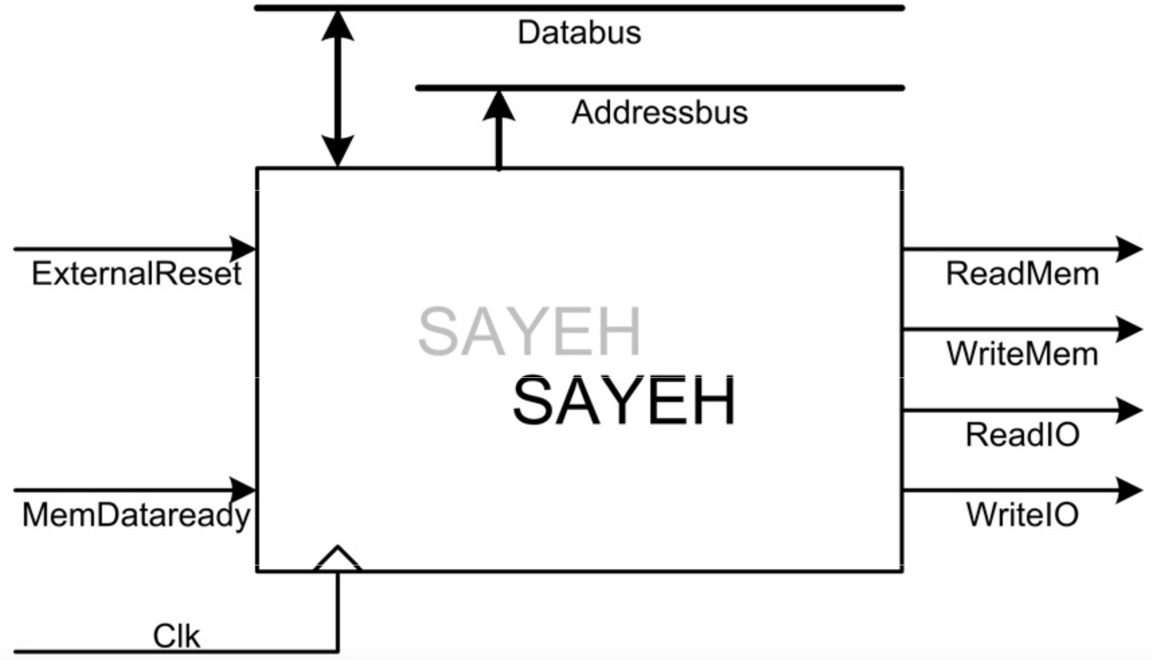
\includegraphics[width=0.75\textwidth]{figs/fig1}\\
	\caption{Sayeh Interface}
\end{figure}

\section{CPU Components}
\subsection{Registerfile}
\par
SAYEH uses it’s \textit{Registerfile} in arithmetic and logical
operations, also addressing modes of the processor take
advantage of this structure, by means of using register file’s
output in addressing calculations. therefore addressing
component of SAYEH has been simplified.

\begin{itemize}
	\item \textbf{Registerfile:} includes 64 registers each of them has  \textbf{16-bit width},
		4 of which are called R0, R1, R2, R3 (note that these four register are not constantly located!
		Think about addressing them by index of 10,11,12,13 now and changing them to 2, 3, 4, 5 in a moment,
		although the location is not constant but they are placed all next to each other, means 2,4,6,7 is not allowed).
	\item \textbf{R0, R1, R2, R3:} as described in register file section, \textbf{(16-bit)}.
\end{itemize}


\subsection{Other Registers}
\par
Alongside \textit{Registerfile} and R0, R1, R2, R3 as a part of that, these registers are also used:

\begin{itemize}
	\item \textbf{Window Pointer(WP):} In order to point to R0 as the base of R0, R1, R2 and R3, Window Pointer is used, (6-bit width).
	\item \textbf{Program Counter(PC):}program counter, (16-bit).
	\item \textbf{Instruction Register(IR):}Instruction Register, which has 16-bit width and would be loaded by a single 16-bit
		instruction or by two 8-bit instructions, (16-bit).
	\item \textbf{Zero Flag(Z):}becomes one when the ALU’s output is zero, (1-bit).
	\item \textbf{Carry Flag(C):} becomes one when the ALU’s output has got carry digit, (1-bit).
\end{itemize}


\subsection{ALU (Arithmetic Logic Unit) Components}
The ALU itself contains these components, each of them is capable of doing the named operation on 16-bit input(s), selecting the desired operation is done by the OPCODE of the instruction.
\begin{itemize}
	\item \textbf{AND Component:}
		This component will perform AND operation on Rs (Source Register) and Rd 			(Destination Register), obviously the result would be another 16-bit vector and 			should be stored in Rd(Destination Register).
	\item \textbf{OR Component:}
		This component will perform OR operation on Rs (Source Register) and Rd (Destination Register), obviously the result would be another 16-bit vector and 			should be stored in destination register.
	\item \textbf{Shift-Right Component(Optional):}
		This component will perform Shift to Right operation on Rs (Source Register) 			obviously the result would be another 16-bit vector and should be stored in 			Rd (destination register).
	\item \textbf{Shift-Left Component:}
		This component will perform Shift to Left operation on Rs (Source Register) 			obviously the result would be another 16-bit vector and should be stored in 			Rd (destination register).
	\item \textbf{Comparison Component:}
		This component will compare Rs and Rd ( if equal then zero flag must become 			one and if Rd is less than Rs then Carry flag (C) would become one)
	\item \textbf{Addition Component:}
		This component will perform Addition between Rs and Rd and Carry flag (C) and 			will store the result in Rd(Destination Register).
	\item \textbf{Subtraction Component:}
		This component will perform Subtraction by means of Rd =Rd-Rs-C.
	\item \textbf{Multiplication Component(Optional):}
		This component will perform Multiplication by means of Rd =Rd*Rs. note that as the multiplication's result of two 8-bit operands would be a 16-bit one so in this processor we will multiply right 8-bits of Rd by right 8-bits of Rs and 16 bit result 			would be stored in Rd.
	\item \textbf{Division Component(Optional):}
		This component will perform Division by means of Rd =Rs/Rd note that just right 		8-bits (Least Significant Bits) of Rd would be used in this action.
	\item \textbf{Square Root Component(Optional):}
		This component will perform Rd= square root(Rs).
	\item \textbf{Random Generator Component(Optional):}
		Generates a random number between 0 to 64000.
	\item \textbf{two’s Complement Component(Optional):}
		Performs two's complement operation on Rs and stores it in Rd(Destination Register).
	\item \textbf{XOR Component(Optional):}
		Just like AND :)
	\item \textbf{Trigonometry Component (sin, cos, tan, cot) by \href{https://en.wikipedia.org/wiki/CORDIC}{CORDIC} IP core(Optional):}
		this component’s extra mark is much more than the other ALU components, 			CORDIC is an IP core used for VHDL (like usual libraries in java,C,...) it’s free and all 			documents could be found on the Internet.
\end{itemize}

\subsection{Other Components}
There is a list of other components needed for the processor to work well and these 		are not embedded into ALU component, such as:
\begin{itemize}
	\item \textbf{No Operation:}
		When this instruction is executed CPU would do nothing for one clock cycle.
	\item \textbf{Halt:}
		By executing this instruction fetching stops for one clock period and the 				previous instruction which has been fetched remains as the last fetched item.
	\item \textbf{Set Zero Flag:}
		This instruction will set zero flag to 1.
	\item \textbf{Clear Zero Flag:}
		When this instruction has been executed zero flag would become 0.
	\item \textbf{Set Carry Flag:}
		This instruction will set carry flag to 1.
	\item \textbf{Clear Carry Flag:}
		When this instruction has been executed carry flag would become 0.
	\item \textbf{Clear Window Pointer:}
		When this instruction has been executed window pointer would become 000000.
	\item \textbf{Move Register:}
		This operation will move the value stored in Rs to Rd.
	\item \textbf{Load Addressed:}
		By this instruction you can load the value stored Rs’th row of memory to Rd.
	\item \textbf{Store Addressed:}
		By this instruction you can store Rs to Rd’th row of memory.
	\item \textbf{Port Manager (Optional):} This component is about to manage ports the SAYEH, SAYEH has 64 ports(named as \textit{P0\ldots to P63}) that should be implemented by you.
		Imagine 64 ports that could be written by the processor and also read by it. these operations would be done by executing instructions like:Input from Port and Output to Port (as mentioned in the Table1).
		Test case of this section would be reading form a desired port and storing it to Rd or reading from Rs and writing it in a desired port.
	\item \textbf{Move Immediate Low:}
		By this instruction 8 bits of \textit{Immediate} operand would be copied to Rd’s left 8 bits (8 least significant bits).
	\item \textbf{Move Immediate High:}
		Exactly like Move \textit{Immediate} Low, but \textit{Immediate} would be stored in most significant bits of Rd.
	\item \textbf{Save PC:} This stores PC to Rd.
	\item \textbf{Jump Addressed:} As shown in Table1.
	\item \textbf{Jump Relative:} As shown in Table1.
	\item \textbf{Branch if Zero:} As shown in Table1.
	\item \textbf{Branch if Carry:} As shown in Table1.
	\item \textbf{Add Win pointer:} As shown in Table1.
\end{itemize}
\section{SAYEH Instructions}
The general format of 8-bit and 16-bit instructions of SAYEH is shown in figure 2. 16-bit 		instructions contains \textit{Immediate} field opposed to 8-bit instructions. The OPCODE field is 	a 4-bit code that specifies the type of the instruction. The \textit{Left} and \textit{Right} is used to 		specify the destination of the operation and \textit{Right} for the source of it (source and 		destination are one of R0 to R3, so within 2 bits we can clarify which is the one we 		desire). The \textit{Immediate} field is used for immediate data if instruction type is 16-bit one, and used for the second 8-bit instruction elsewhere.

\begin{figure}[ht]
	\centering
	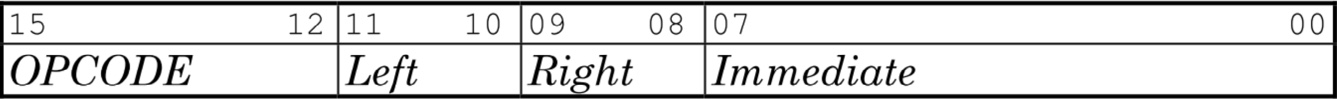
\includegraphics[width=0.75\textwidth]{figs/fig2}
	\caption{Sayeh Instructions Format}
\end{figure}

\par
Our processor (SAYEH) has total of 35 instructions  some of which are optional. Instructions within 16-bit length are the ones contains \textit{Immediate} field and others don’t. Instructions that use destination and source fields (shown as D and S in the table of instructions set) have an OPCODE limited to 4 bits. Instructions that don’t require specification of source and destination registers use these fields as OPCODE extensions. Finally the overview of SAYEH’s instruction set would be as shown in table1 (note that some of optional parts hasn’t been mentioned in this table and Mnemonic and bit vector representation of them should be designed by you).
\par
In the instruction set, addressed locations in the memory are indicated by enclosing the address in a set of parenthesis (instructions like load addressed or store addressed). For these instructions, the processor issues ReadMem or WriteMem signals to the memory. When input and output instructions (input, output) are executed, SAYEH issues ReadIO or WriteIO signals to its IO devices.

\begin{table}[H]
	\centering
	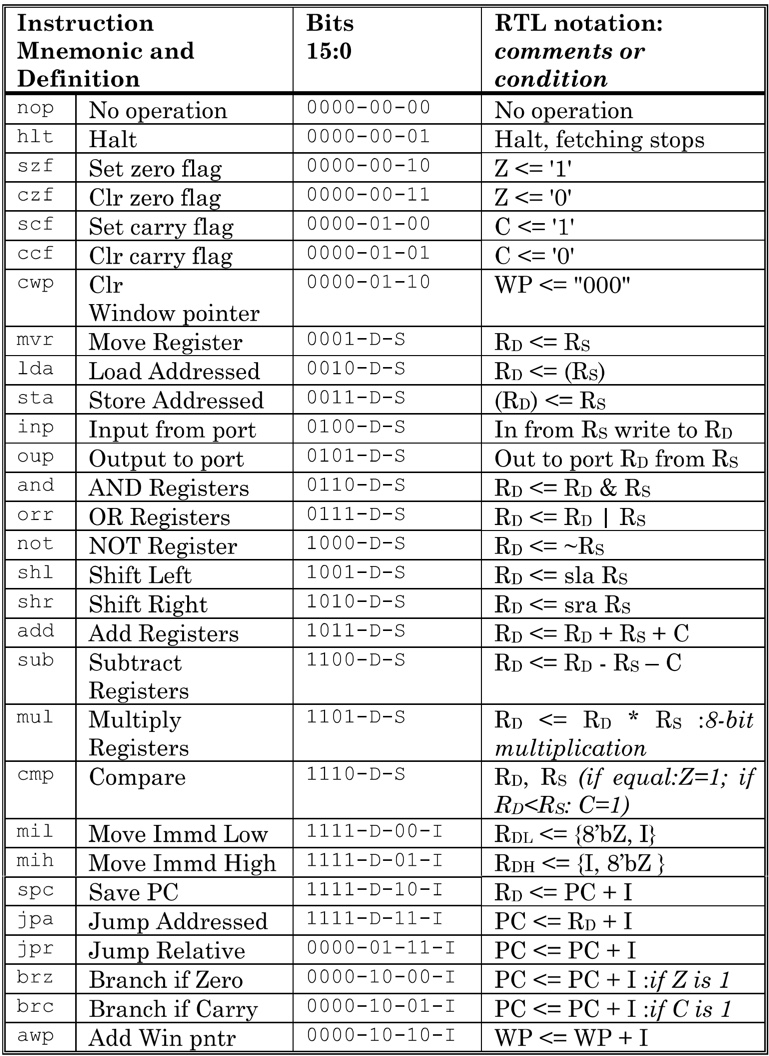
\includegraphics[width=0.75\textwidth]{figs/table1}\\
	\caption{Instruction Set of SAYEH}
\end{table}

\section{Datapath}
The datapath of SAYEH is shown in Figure 3. The main components of this machine are the followings:
\begin{itemize}
	\item \textbf{PC (Program Counter)}
	\item \textbf{Address Logic}
	\item \textbf{IR (Instruction Register)}
	\item \textbf{WP (Window Pointer)}
	\item \textbf{Register File}
	\item \textbf{ALU(Arithmetic Logic Unit)}
	\item \textbf{Flags}
\end{itemize}

\par As shown in figure 3 these components are either hardwired or connected through three state buses. Component inputs with multiple sources, such as the right hand side input of ALU, use three-state buses. Three-state busses in this structure are Databus and OpndBus . In this figure, signals that are in italic are control signals issued by the controller. These signals control register clocking, logic unit operations and placement of data in busses.

\begin{figure}[ht]
	\centering
	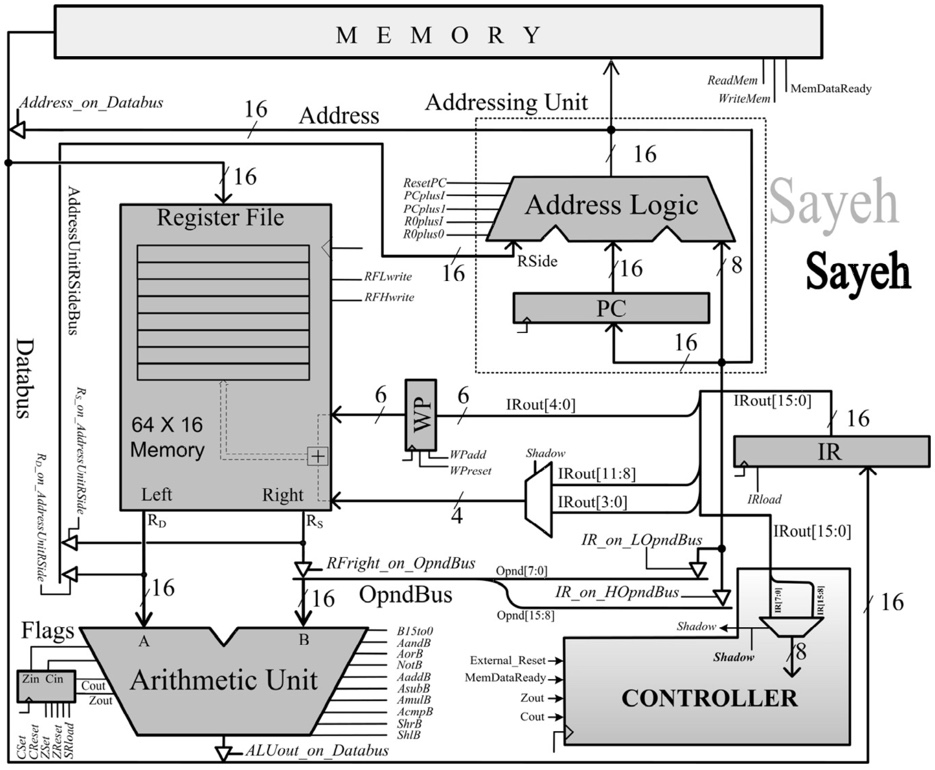
\includegraphics[width=0.99\textwidth]{figs/fig3}\\
	\caption{SAYEH Datapart}
\end{figure}

\subsection{Datapath Components}
Figure 4 shows the hierarchical structure of SAYEH components. The processor has a Datapath and a Controller. Datapath components are Addressing Unit, IR Module, WP, Register File, Arithmetic Logic Unit (ALU), and the Flags register. The Addressing Unit is further partitioned into the PC and Address Logic.
\par
The Address Logic is a combinational circuit that is capable of adding its inputs to generate a 16-bit output which represents the address of the row we are about to fetch from memory. Register File is a two-port memory and a file of 64 16-bit registers. The Window Pointer is a 6-bit register that is used as the base of the Register File. Specific registers for read and write (R0, R1, R2 or R3) in the Register File are selected by its 4-bit input bus coming from the Instruction Register. Two bits select the source and another two selects the destination (means all of our operands, except \textit{Immediate} ones are one of R0, R1, R2 or R3 selected by the mentioned signal).
\par
When the Window Pointer add is enabled, it adds its 6-bit input to its current data. The Flags Register is a 2-bit register that saves the flag outputs of the Arithmetic Unit . The Flags Register is a 2bit register that saves the flag outputs of the Arithmetic Unit. The Arithmetic Unit is a 16-bit arithmetic and logic unit that has logical, shift, add and compare operations and … (as discussed in it's own section). A 9-bit input selects one of the nine functions of the ALU. This code is provided by the SAYEH’s controller component.
\begin{figure}[ht]
	\centering
	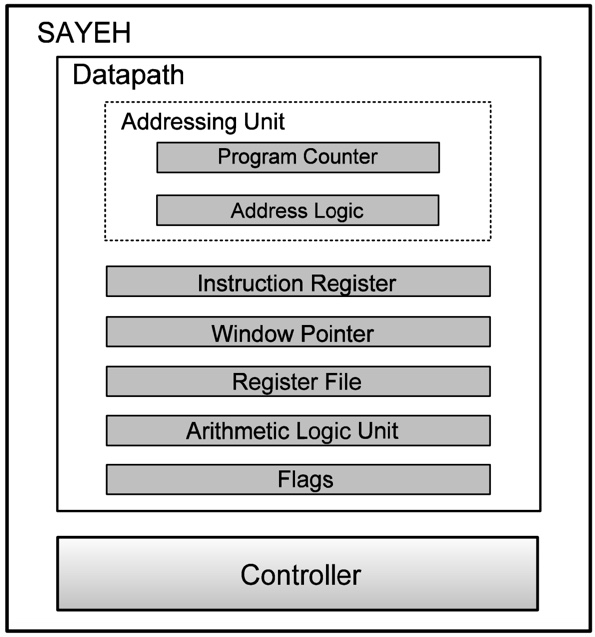
\includegraphics[width=0.68\textwidth]{figs/fig4}\\
	\caption{Sayeh Hierarchical Structure}
\end{figure}

\par
Controller Component of SAYEH has eleven states for various reset, fetch, decode, execute and halt operations. Signals generated by the controller control logic unit operations and register clicking in the data-path.
\par
SAYEH sequential data components and its controller are triggered on the rising-edge of the main system clock. Control signals remain active after one rising edge through the next.This duration allows for propagation of signals through the busses and logic units in the data-path.


\section{SAYEH VHDL Description}
SAYEH should be described according to the hierarchical structure of Figure4. Data components should be described separately, and then wired to each other from the datapath component. Controller is described in a single VHDL module. In the complete SAYEH description, the datapath and controller are wired together.
\subsection{Data Components}
Combinational and sequential SAYEH data components are partially described here. The combinational ones are like the ALU that performs arithmetic and logical operations. The function of such units is controlled by the controller. The sequential components are clocked with the negative edge of the main CPU clock. These components have functionalities like loading and resetting and are controlled by the controller.
\subsubsection{Addressing Unit}
The Addressing Unit of figure 5 consists of the Program Counter and Address Logic. The Program Counter is a simple register with enabling and resetting mechanisms, whhile the Address Logic is a small arithmetic unit that performs adding and incrementing for calculating PC or memory addresses.
\par
This unit has a 16-bit input coming from the Register File, an 8-bit input from the Instruction Register, and a 16-bit address output. Control signals of the Addressing Unit are \textit{ResetPC, PCplusI, PCplus1, RplusI, Rplus0,} and \textit{PCenable}. These control signals select what goes on the output of this unit. Shown in Figure 6 is the VHDL code of the Program Counter. The Address Logic of Figure7 uses control signal inputs of the Addressing Unit to generate input data to the Program Counter via the PCout of Figure 5. Constants defined and used here correspond to one-hot control signals from the controller.

\begin{figure}[H]
	\centering
	\begin{minted}
	[
	fontsize=\footnotesize,
	linenos
	]{vhdl}
	ENTITY AddressUnit IS
	    PORT (
		Rside : IN std_logic_vector (15 DOWNTO 0);
		Iside : IN std_logic_vector (7 DOWNTO 0);
		Address : OUT std_logic_vector (15 DOWNTO 0);
		clk, ResetPC, PCplusI, PCplus1 : IN std_logic;
		RplusI, Rplus0, EnablePC : IN std_logic
	    );
	END AddressUnit;

	ARCHITECTURE dataflow OF AddressUnit IS
	    COMPONENT pc . . . END COMPONENT;
	    COMPONENT al . . . END COMPONENT;

	    SIGNAL pcout : std_logic_vector (15 DOWNTO 0);
	    SIGNAL AddressSignal : std_logic_vector (15 DOWNTO 0);
	BEGIN
	    Address <= AddressSignal;
	    l1 : pc PORT MAP (EnablePC, AddressSignal, clk, pcout);
	    l2 al PORT MAP
		(pcout, Rside, Iside, AddressSignal,
		ResetPC, PCplusI, PCplus1, RplusI, Rplus0);
	END dataflow;
	\end{minted}
	\caption{\textit{Addressing Unit} VHDL code}
\end{figure}

\begin{figure}[H]
	\centering
	\begin{minted}
	[
	fontsize=\footnotesize,
	linenos
	]{vhdl}
	ENTITY ProgramCounter IS
	    PORT (
		EnablePC : IN std_logic;
		input: IN std_logic_vector (15 DOWNTO 0);
		clk : IN std_logic;
		output: OUT std_logic_vector (15 DOWNTO 0);
	    );
	END ProgramCounter;

	ARCHITECTURE dataflow OF ProgramCounter IS BEGIN
	    PROCESS (clk) BEGIN
		IF (clk = '1') THEN
		    IF (EnablePC = '1') THEN
			output <= input;
		    END IF;
		END IF;
	    END PROCESS;
	END dataflow;
	\end{minted}
	\caption{\textit{Program Counter} VHDL code}
\end{figure}

\begin{figure}[H]
	\centering
	\begin{minted}
	[
	fontsize=\footnotesize,
	linenos
	]{vhdl}
	ENTITY AddressLogic IS
	    PORT (
		PCside, Rside : IN std_logic_vector (15 DOWNTO 0);
		Iside : IN std_logic_vector (7 DOWNTO 0);
		ALout : OUT std_logic_vector (15 DOWNTO 0);
		ResetPC, PCplusI, PCplus1, RplusI, Rplus0 : IN std_logic
	    );
	END AddressLogic;

	ARCHITECTURE dataflow of AddressLogic IS
	    CONSTANT one   : std_logic_vector (4 DOWNTO 0)
			   := "10000"
	    CONSTANT two   : std_logic_vector (4 DOWNTO 0)
			   := "01000"
	    CONSTANT three : std_logic_vector (4 DOWNTO 0)
			   := "00100"
	    CONSTANT four  : std_logic_vector (4 DOWNTO 0)
			   := "00010"
	    CONSTANT five  : std_logic_vector (4 DOWNTO 0)
			   := "00001"
	BEGIN
	    PROCESS (PCside, Rside, Iside, ResetPC,
		    PCplusI, PCplus1, RplusI, Rplus0)
		VARIABLE temp : std_logic_vector (4 DOWNTO 0);
	    BEGIN
		temp := (ResetPC & PCplusI & PCplus1 & RplusI & Rplus0);
		CASE temp IS
		    WHEN one => ALout <= (OTHERS => '0');
		    WHEN two => ALout <= PCside + Iside;
		    WHEN three => ALout <= PCside + 1;
		    WHEN four => ALout <= Rside + Iside;
		    WHEN five => ALout <= Rside;
		    WHEN OTHERS => ALout <= PCside;
		END CASE;
	    END PROCESS;
	END dataflow;
	\end{minted}
	\caption{\textit{Address Logic} VHDL code}
\end{figure}

\subsubsection{Memory}
You need to use memory module as a storage. we design this unit for you and you
can instantiate this module in your datapath. for using this module you just put
it's entity as component and pass arrays with correct size to it, it works :)

\begin{figure}[H]
	\centering
	\begin{minted}
	[
	fontsize=\footnotesize,
	linenos
	]{vhdl}
	entity memory is
		port (address : in std_logic_vector;
			data_in : in std_logic_vector;
			data_out : out std_logic_vector;
			clk, rwbar : in std_logic);
	end entity memory;
	\end{minted}
	\caption{\textit{Memory} VHDL entity code}
\end{figure}

Source codes avaiable \href{https://github.com/AUT-CEIT/Arch101/blob/master/memory/memory.vhd}{here}.

\section{Important Notes}

\begin{enumerate}
	\item
		All your project should be implemented by VHDL not Verilog or\ldots
	\item
		A part of your score would be devoted to the report you deliver within your projects code. In this report you would explain the whole job and anything special you have done. (note that it shouldn't be shorter than this document and should be typed!)
	\item
		Controller should be designed by an Finite State Machine (FSM) and this FSM should be mentioned in your project report.
	\item
		Name of your modules, OPCODEs,\ldots should be exactly the same as the ones mentioned in this document.
	\item
		In addition to bonus sections mentioned beforehand, implementation of this project on \textit{Altera DE2} FPGA boards will result in extra mark as well.
	\item
		You can simulate your code with softwares like: Modelsim, Altera Quartus, GHDL, Xilinx ISE, Active HDL, Xilinx Vivado Design Suite,\ldots (note that Modelsim and Quartus has got free versons and GHDL is totally free so it's better to obey \textit{Copyright}) but the TA's laptop is only equipped with Modelsim and in case of delivery you should be able of running your code in that environment.
	\item
		Place all your modules and report into a .zip file named as "FirstName LastName StudentID" before upload. if any other module is used in your implementation but hasn't been mentioned in this document place it in it's proper place next to modules within the same hierarchy.
	\item
		This project could be done both individually and in a group:
		\begin{itemize}
			\item \textbf{Individual:}
				\begin{enumerate}
					\item
						your score which is out of 100 would be multiplied by 1.2.

				\end{enumerate}
			\item \textbf{As a member of a group:}
				\begin{enumerate}
					\item
						your score which is out of 100 would be multiplied by 0.9.
					\item
						We assume each of the two members had been involved in every single line of project so the project would be delivered individually.
				\end{enumerate}
		\end{itemize}

	\item
		In case of delivery, your code will be downloaded by the responsible TA from Moodle, so the only way to convay your code is Moodle and in if you need to reform your code please upload it when possible to be used in the due date.
	\item
		\textbf{Cheating Alert!}
		\begin{enumerate}
			\item
				All your codes would be processed, both manually and automatically and in case of any similarity by any means, both of individuals involved, would be fined by getting -35 percent of the project's score (note that if pushing your code to Github or any other VCS, exposing your code to a friend or \ldots results in unexpected similarities of others, you ALL, are responsible!).
			\item
				Any cooperation beyond members of the group is forbidden!
			\item
				The only source you are allowed to copy form, is AUT/CEIT/Arch101 reposetory which has been devoted to this course.
		\end{enumerate}
	\item All questions would be answered by the course's email: computerarchitecture95@gmail.com.
\end{enumerate}


\end{document}



